%%%%%%%%%%%%%%%%%%%%
%% 04-RESULTS %%
%%%%%%%%%%%%%%%%%%%%
\clearpage\section{Implementation and results}

In this chapter we will explain the different use cases that our framework provides along with the programs captures of the tools explained in chapter 3.
\TODO{provide the cite etc para el chapter}

We will explain one workflow for each tool.

\subsection{lxce}
For the first workflow, we will explain how to initiliaze the command and manage some containers configurations.

In specific we will:
\begin{itemize}
	\item{Initialize the command}
	\item{Create some containers}
	\item{Change linux distributions for containers}
	\item{Delete some containers}
	\item{Add and delete proxies on containers}
	\item{Delete the command and configurations}
\end{itemize}

%%% INITIALIZE COMMAND %%%
\textbf{Initialize the command}
The first thing we have to do is initizalie the command in order to generate the default configurations files and select different parameters.

\begin{minted}[bgcolor=background]{text}
root@oscar-vm: # lxce init
? lxce.conf: Select hypervisor hostname: oscar-vm
? lxce.conf: Select ssh suffix: gold
? lxce.conf: Select vnc server: localhost
? lxce.conf: Select vnc port: 5901
? lxce.conf: Select data location [full path]: /datasdd
? Want to add another data location (just hit enter for YES)? No
? container.default: Select containers base: ubuntu:20.04
? container.default: Select default container location: /datasdd
[] Good!
root@oscar-vm: #
\end{minted}

That results in the following:
\begin{minted}[bgcolor=background]{text}
/etc/lxce 
|--- container.conf.d 			
|--- container_default.conf 		
|--- lxce.conf 			
|--- remmina 		
'--- ssh 	
\end{minted}
with the configurations files:
\begin{minted}[bgcolor=background]{text}
root@oscar-vm:~# cat /etc/lxce/lxce.conf
{
  "hypervisor": {
    "SSH_hostname": "oscar-vm",
    "SSH_suffix": "gold",
    "VNC_server": "localhost",
    "VNC_port": 5901
  },
  "seed": "58afb0f0250a8eb4",
  "domains": [
    {
      "id": 0,
      "name": "default"
    }
  ],
  "locations": [
    "/datasdd"
  ]
}
root@oscar-vm:~# cat /etc/lxce/container_default.conf
{
  "name": "",
  "alias": "",
  "user": "",
  "id_domain": 0,
  "id_container": 0,
  "domain": "default",
  "base": "ubuntu:20.04",
  "userData": "/datasdd",
  "proxies": [
    {
      "name": "ssh",
      "type": "tcp",
      "listen": "0.0.0.0",
      "port": 22
    },
    {
      "name": "test",
      "type": "tcp",
      "listen": "0.0.0.0",
      "port": 3000
    }
  ],
  "nginx": {
    "novnc": 7000,
    "www": 80
  }
}
\end{minted}

%%% CREATE SOME CONTAINERS %%%
\textbf{Create containers}
Then we can create 3 containes with different alias in the domain test with:
\begin{minted}[bgcolor=background]{text}
root@oscar-vm:~# lxce launch -r 3 -d test -a alice bob peter 
[*] --------------------------------------------------------------
[*] Checking ...
[*] Initialized
[*] Initialized: ok!
[*] Access
[*] Access: ok!
[*] Checks: ok!
[*] --------------------------------------------------------------
[*] Launching container with managing-harlequin
[**] launching ...
[**] waiting for container...
[**] Getting user
[**] Getting user: ubuntu !!
[**] Password created: fa89a2eaca
[**] launching: ok!
[**] creating configurations
[**] creating configurations: ok!
[**] read only directories
[**] added data-test shared folder
[**] added data-managing-harlequin shared folder
[**] read only directories: ok!
[**] adding proxies
[**] added proxy-ssh
[**] added proxy-test
[**] adding proxies: ok!
[**] dns resolution: managing-harlequin.lxd -> 10.10.1.171
[] Launching container with managing-harlequin
[*] Launching container with excited-amethyst
...
...
[] Launching container with excited-amethyst
[*] Launching container with coloured-purple
....
....
[] Launching container with coloured-purple
[*] --------------------------------------------------------------
[*] Success!!
\end{minted}
Where we can see the containers created, along with their properties, with:

\begin{figure}[H]
\label{fig:lxce list}
\centering
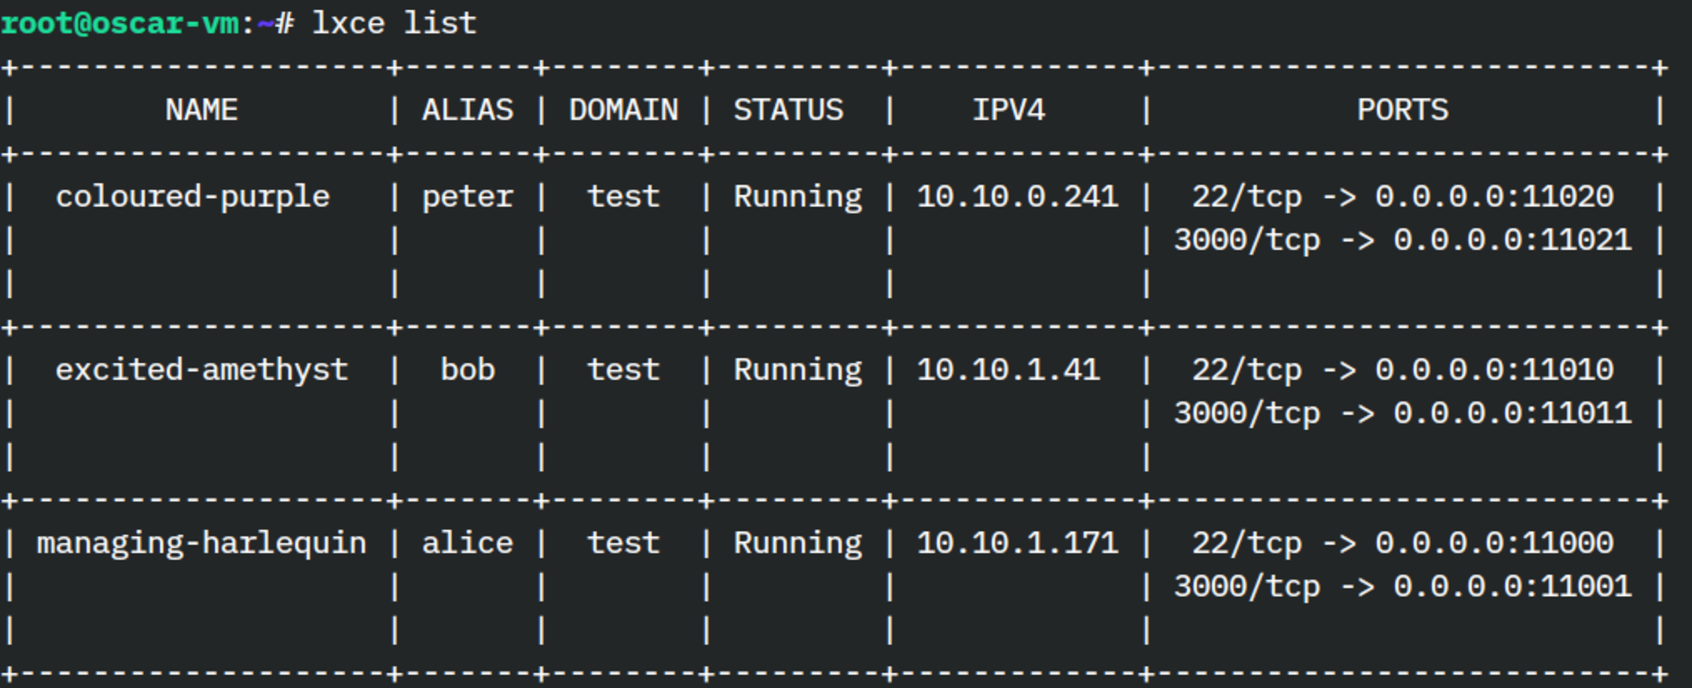
\includegraphics[width=\textwidth]{img/04/lxce-list.pdf}
\caption[Prototype setup]{\footnotesize{lxce list.}}
\end{figure}

%%% CHANGE CONTAINER BASES %%%
\textbf{Change container base}
We have set up all the containers to be run with ubuntu:20.04 base, but if we we would like to change one container (peter for example) to use ubuntu:18.04 instead we could do it by:
\begin{minted}[bgcolor=background, breaklines]{text}
root@oscar-vm:~/m/tfg-lxce# lxce rebase -d test -a peter -b ubuntu:18.04
? Do you want to rebase coloured-purple container within test with ubuntu:18.04? Yes
[*] Rebasing coloured-purple
[**] Removing coloured-purple
[**] launching container with base: ubuntu:18.04 ...
[**] waiting for container
[**] Getting user
[**] Getting user: ubuntu !!
[**] added proxy-ssh
[**] added proxy-test
[**] added data-ubuntu
[**] added data-test
[**] dns resolution: coloured-purple.lxd -> 10.10.0.168
[] Rebasing coloured-purple
\end{minted}
where all the properties of the container will remain the same.

So then we would have the following:
\begin{minted}[bgcolor=background]{text}
root@oscar-vm:~/m/tfg-lxce# lxce list -c nadb
+--------------------+-------+--------+--------------+
|        NAME        | ALIAS | DOMAIN |     BASE     |
+--------------------+-------+--------+--------------+
|  coloured-purple   | peter |  test  | ubuntu:18.04 |
+--------------------+-------+--------+--------------+
|  excited-amethyst  |  bob  |  test  | ubuntu:20.04 |
+--------------------+-------+--------+--------------+
| managing-harlequin | alice |  test  | ubuntu:20.04 |
+--------------------+-------+--------+--------------+
\end{minted}

\subsection{lxce-admin}
\subsection{web-admin}

\TODO{Hello, world\today}


